% Asset ID: AS2ForcesAndNewtonsLawsTikZ-006
% Source: Chapter 10 Forces and Motion evidence; CCEA AS2-FORCES boundary
% Related section: Vector F equals ma
% Purpose: Vector F equals ma.

\documentclass[tikz,border=6pt]{standalone}
\usetikzlibrary{arrows.meta,positioning}
\begin{document}
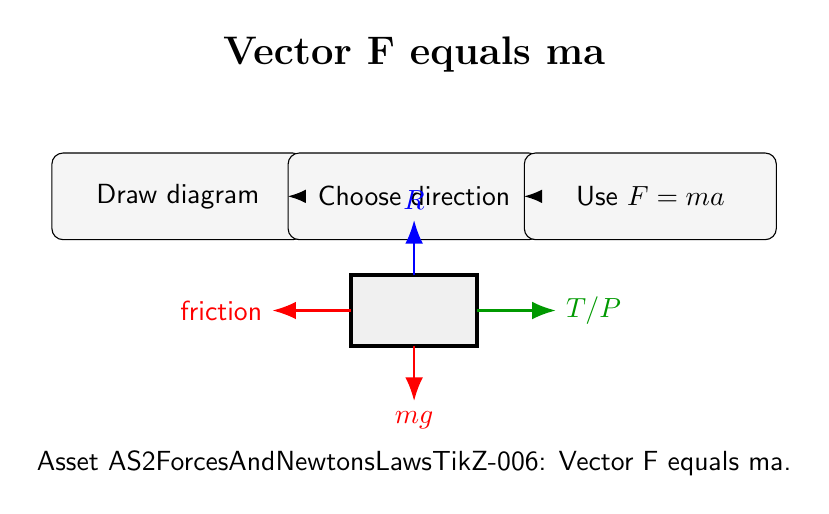
\begin{tikzpicture}[>=Latex,font=\sffamily,box/.style={draw,rounded corners,fill=gray!8,align=center,minimum width=3.2cm,minimum height=1.1cm},force/.style={-{Latex[length=3mm]},thick}]
\node[font=\bfseries\Large] at (0,3.2) {Vector F equals ma};
\node[box] (a) at (-3,1.4) {Draw diagram};
\node[box] (b) at (0,1.4) {Choose direction};
\node[box] (c) at (3,1.4) {Use $F=ma$};
\draw[->,thick] (a) -- (b);
\draw[->,thick] (b) -- (c);
\draw[very thick,fill=gray!12] (-0.8,-0.5) rectangle (0.8,0.4);
\draw[force,blue] (0,0.4)--(0,1.1) node[above] {$R$};
\draw[force,red] (0,-0.5)--(0,-1.2) node[below] {$mg$};
\draw[force,green!60!black] (0.8,-0.05)--(1.8,-0.05) node[right] {$T/P$};
\draw[force,red] (-0.8,-0.05)--(-1.8,-0.05) node[left] {friction};
\node[align=center] at (0,-2.0) {Asset AS2ForcesAndNewtonsLawsTikZ-006: Vector F equals ma.};
\end{tikzpicture}
\end{document}
